% ****** Start of file apssamp.tex ******
%
%   This file is part of the APS files in the REVTeX 4.2 distribution.
%   Version 4.2a of REVTeX, December 2014
%
%   Copyright (c) 2014 The American Physical Society.
%
%   See the REVTeX 4 README file for restrictions and more information.
%
% TeX'ing this file requires that you have AMS-LaTeX 2.0 installed
% as well as the rest of the prerequisites for REVTeX 4.2
%
% See the REVTeX 4 README file
% It also requires running BibTeX. The commands are as follows:
%
%  1)  latex apssamp.tex
%  2)  bibtex apssamp
%  3)  latex apssamp.tex
%  4)  latex apssamp.tex
%
\documentclass[%
 reprint,
%superscriptaddress,
%grouhttps://www.overleaf.com/project/62e7efbe949d9b3fb167d1cdpedaddress,
%unsortedaddress,
%runinaddress,
%frontmatterverbose, 
%preprint,
%preprintnumbers,
%nofootinbib,
%nobibnotes,
%bibnotes,
 amsmath,amssymb,
 aps,
%pra,
%prb,
%rmp,
%prstab,
%prstper,
%floatfix,
]{revtex4-2}

\usepackage{graphicx}% Include figure files
\usepackage{dcolumn}% Align table columns on decimal point
\usepackage{bm}% bold math
\usepackage{amsmath,amssymb,amsfonts}
\usepackage{algorithmic}
\usepackage{tabularx}
\usepackage{xcolor}
\usepackage{array}  
    \newcolumntype{L}{>{\raggedright\arraybackslash}X}
\newcolumntype{P}[1]{>{\centering\arraybackslash}p{#1}}
%\def\BibTeX{{\rm B\kern-.05em{\sc i\kern-.025em b}\kern-.08em
%    T\kern-.1667em\lower.7ex\hbox{E}\kern-.125emX}}
%\usepackage{hyperref}% add hypertext capabilities
%\usepackage[mathlines]{lineno}% Enable numbering of text and display math
%\linenumbers\relax % Commence numbering lines

%\usepackage[showframe,%Uncomment any one of the following lines to test 
%%scale=0.7, marginratio={1:1, 2:3}, ignoreall,% default settings
%%text={7in,10in},centering,
%%margin=1.5in,
%%total={6.5in,8.75in}, top=1.2in, left=0.9in, includefoot,
%%height=10in,a5paper,hmargin={3cm,0.8in},
%]{geometry}

\begin{document}

\preprint{APS/123-QED}

\title{Spurious Solar-Wind Effects on Acceleration Noise in LISA Pathfinder}% Force line breaks with \\
\author{Arnold Yang\(^1\)}%
\author{Indie Desiderio-Sloane\(^1\)}
 \author{Grant David Meadors\(^2\)}

\affiliation{%
Institute for Computing in Research\(^1\)
 Los Alamos National Laboratory\(^2\)
}%

\date{\today}% It is always \today, today,
             %  but any date may be explicitly specified

\begin{abstract}
Spurious solar-wind effects may contribute as a candidate noise factor on the precise instrumentation of the future Laser Interferometer Space Antenna(LISA). To predict the possible impact of this noise factor, models were used to display spurious solar wind effects on acceleration noise in LISA Pathfinder. Data from NASA's Advanced Composition Explorer(ACE) which was also situated at the L1 Lagrange point was used as a reliable source of Solar Wind data. To test this, the data from both satellites was formatted, gap-filled and adapted for comparison and a coherence plot was created comparing the results of the fast Fourier transformations. The coherence plot suggested that Solar Wind had a minuscule effect on the LPF and higher frequency coherence(LISA’s main observing band) can be attributed to random chance correlation. This result is encouraging for the future LISA project as this suggests higher instrumentation accuracy and that solar wind is not a major source of noise. 
\end{abstract}

%\keywords{Suggested keywords}%Use showkeys class option if keyword
                              %display desired
\maketitle

%\tableofcontents

\section{introduction}
The future Laser Interferometer Space Antenna (LISA) will be the first space-based gravitational wave detector on a heliocentric orbit, capable of detecting lower frequencies than Laser Interferometer Gravitational Wave Observatory (LIGO). To test the LISA concept, an early satellite the LISA Pathfinder (LPF) was sent up with similar equipment to the future LISA. LPF used 2 pure free-falling masses at which the accelerations at the femto-g level could be measured, the same level at which minute gravitational wave passes can be detected[5]. To ensure reliability a control system was introduced to keep the test masses centered in the spacecraft[4]. With such precise instrumentation the control system is designed to counteract a multitude of disturbances including solar wind/irradiance, micrometeoroids, and gravity from other interstellar mass. The LPF flew no instrumentation to measure the spurious solar wind effect. Therefore using current solar wind satellite the Advanced Composition Explorer(ACE), various plots were made comparing 1,684 hours of LPF and ACE data across a 114 day time span to estimate the effects of solar wind on the LISA.\\

\begin{figure}[htbp]
\centerline{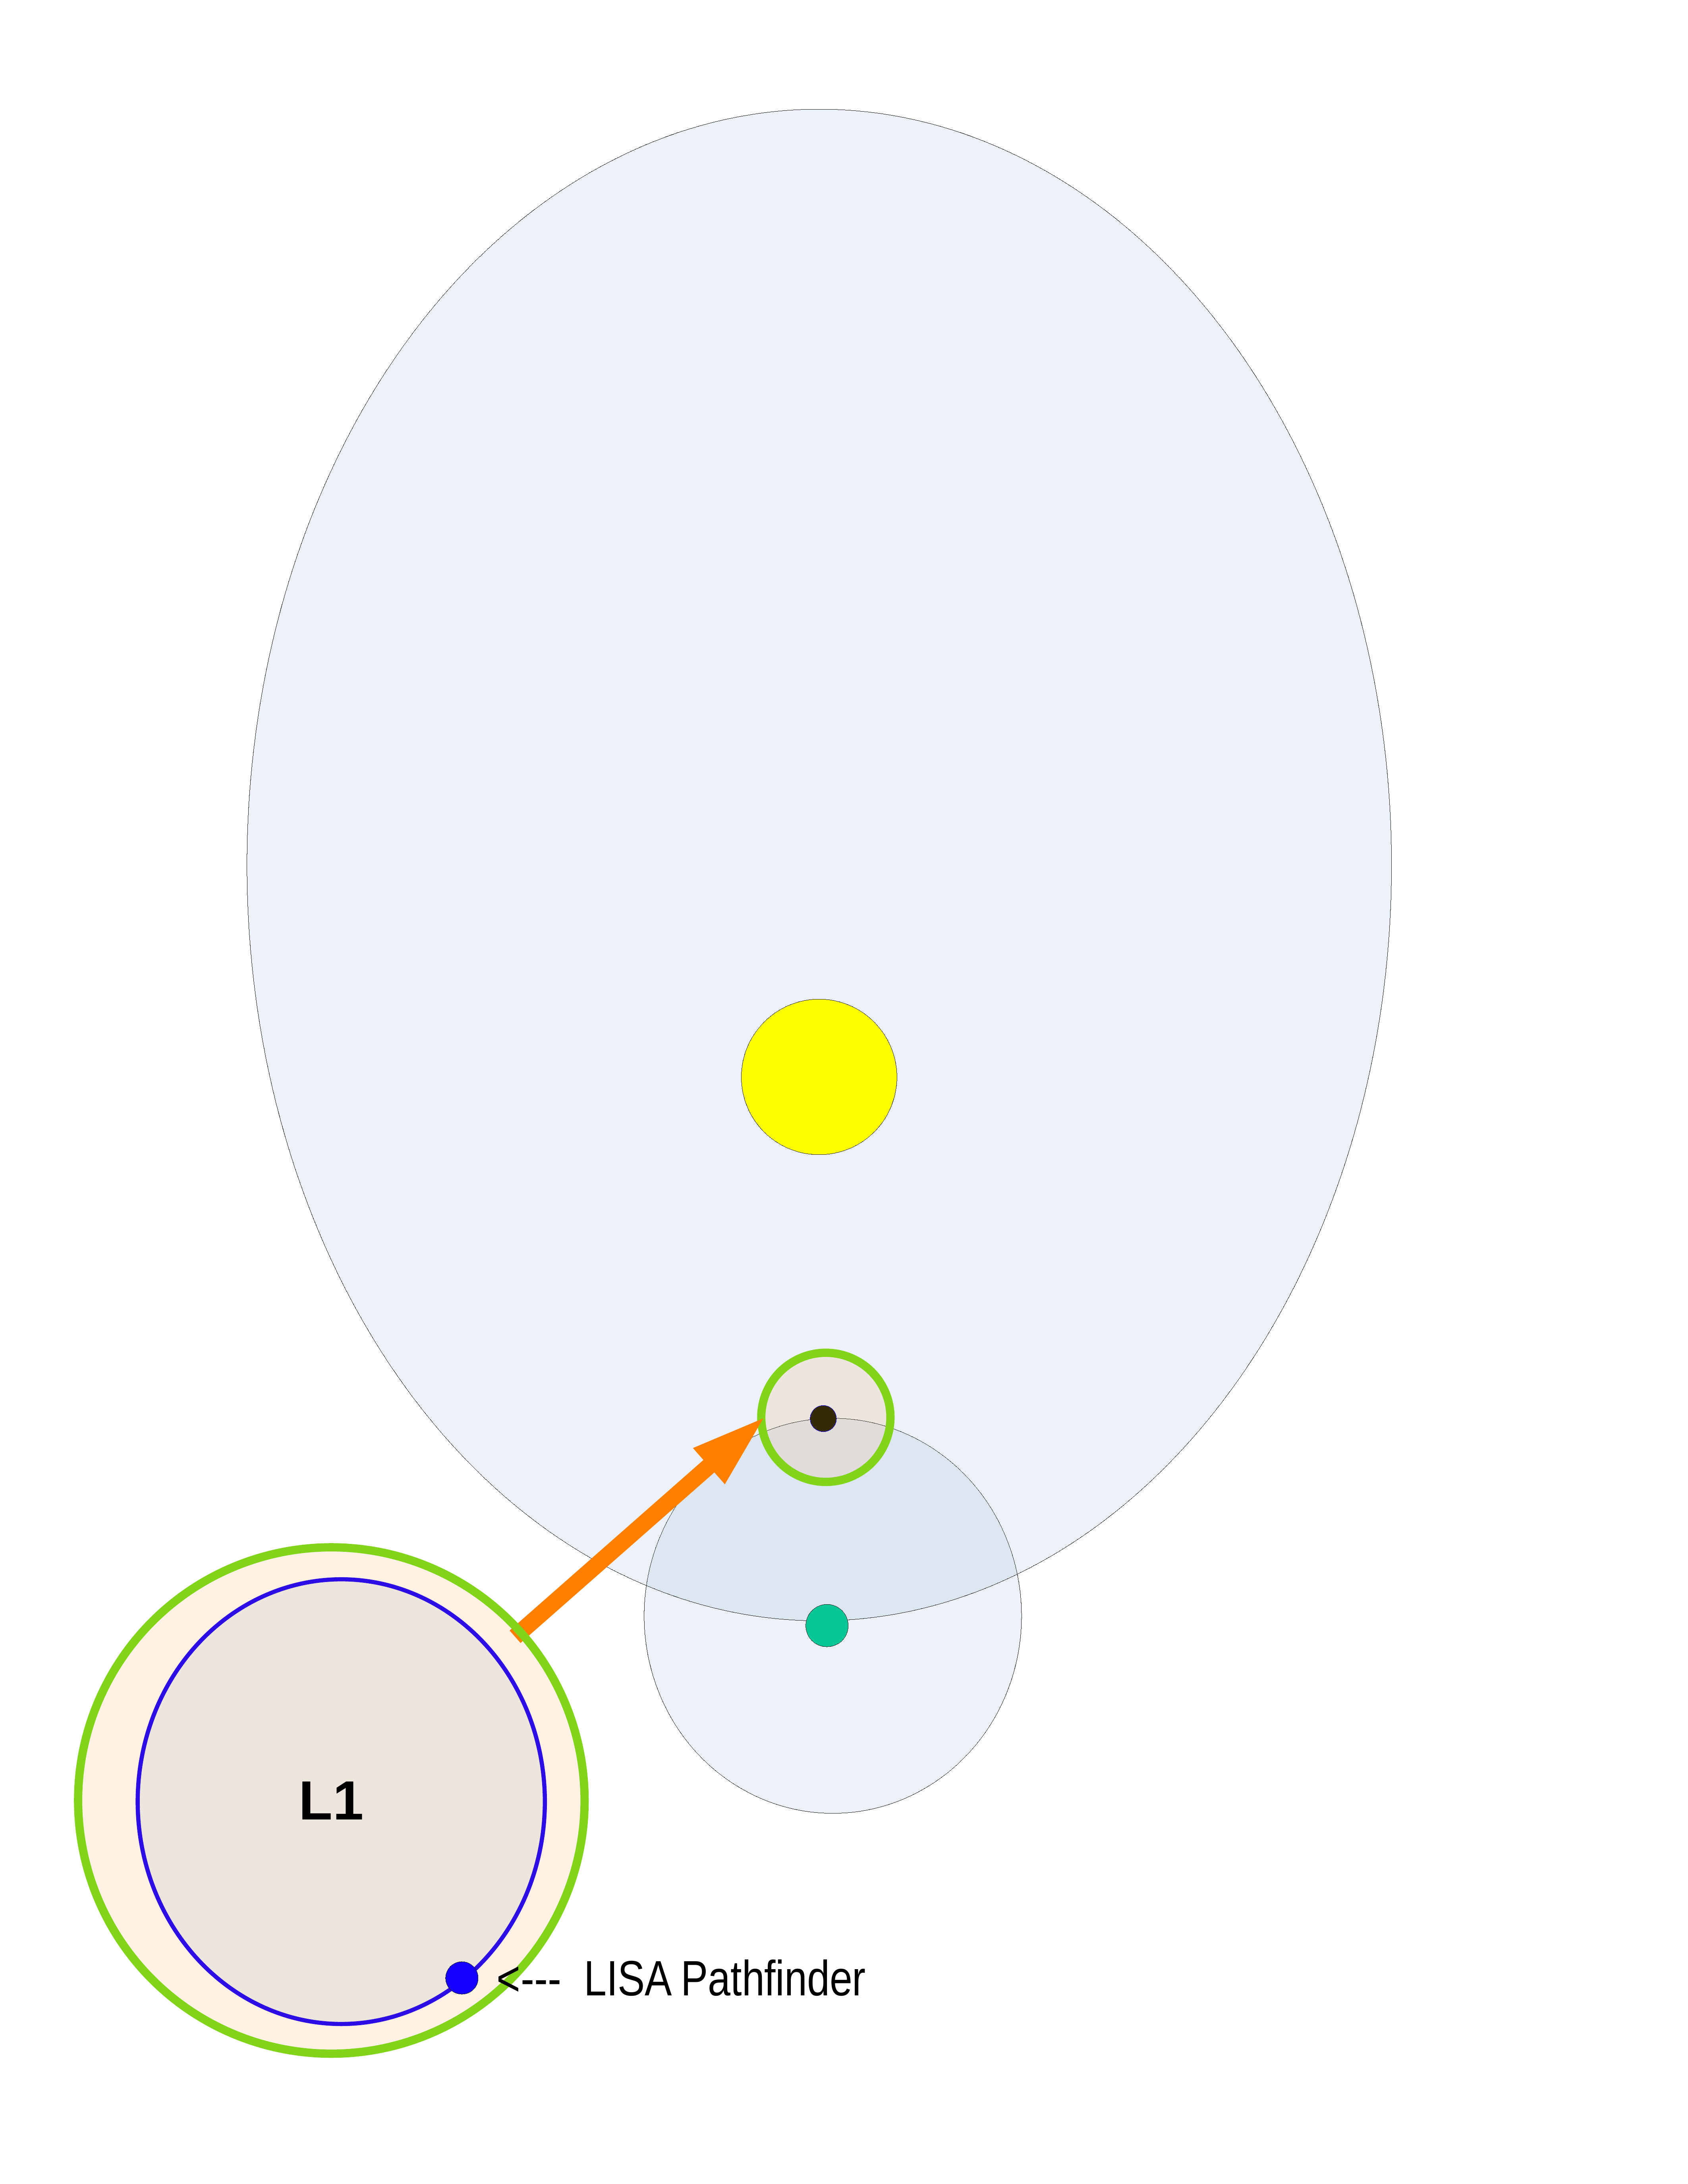
\includegraphics[width=0.5\textwidth]{pathfinder_orbit_model-1.png}}
\caption{This diagram shows the positioning of the LISA Pathfinder in relation to the Sun and Earth.}
\label{fig}
\end{figure}

Solar wind originates from the Sun's corona and consists of charged particles. Bursts of particles can be emitted in events known as coronal mass ejections (CMEs). The emitted high speed charged particles can reach speeds of 800 kilometers per second, larger storms have been known to be damaging to satellite function and are known causes for inaccuracy of GPS satellites. The charges of these particles have a lesser effect on the LPF satellite, however, solar wind may contribute to a small force on the movement of this mass which contributes to noise in the data.\\

The following paper is as is, section II [name] we summarize the procedure of formatting and transforming ACE and LISA data to be compared. Section III [name] will detail the results, and conclusions and all future implications are contained in Section IV. \\

\subsection{\label{sec:level2}Related Works}
Spatial weather has been identified as a key noise factor in possible future LISA measurements. Past work in assessing the impact involved using SOHOs Virgo Solar irradiance and ACE Solar Wind data to model possible impacts on the future LISA space antenna (Frank et al. 2020).
Another major source of noise identified for LPF is micrometeoroids and through various models 54 impact candidates were identified across a 4348 hour time period and were shown to be similar to those resulting from Jupiter Family Comets (JFC), Oort cloud comets, Halley-type comets, and asteroids[4]. 
Additionally, the creation of LISA is renewing the interest in the environment of space. This environment includes solar energetic particles, galactic cosmic ray fluxes, and the effects of solar neutrons and interplanetary electrons[2]. 

\section{Methods}
This section describes the steps taken to format, compile, and plot data from ACE and LPF.
\begin{figure}[htbp]
\centerline{
\includegraphics[width=0.5\textwidth]{fig1solWmam.jpg}}
\caption{Flow diagram for steps taken}
\label{fig}
\end{figure}
\subsection{ACE data-Formatting, Filtering, Gap Filling, Calculations
}
We used solar wind data from the Advanced Composition Explorer (ACE), which provided solar wind velocity components, alpha particle to proton ratios, proton densities at 64 second intervals measured in UTC time[3]. Further formatting required converting UTC time to the GPS time format used by LPF data and filtering and gap filling all bad data values (-9999.9 as specified in the ACE data file header)[3]. The gaps were separated into 3 categories by length using the method of gap fill from \textit{Modeling Spurious Forces on the LISA Spacecraft Across a Full Solar Cycle} [1], for best effect when fast Fourier transformation(FFT) is used. Type A gaps are of length 1 and can be filled with simple linear interpolation  (averaging values on either side of the graph). Type B gaps are of lengths between 2 and 24 and filled with a combination of Gaussian Noise and linear interpolation. For the Gaussian noise (\(\sigma\)) to have similar characteristic to the data around it, \(\sigma_{1}\) and \(\sigma_{2}\) are the standard deviations sampling data of equal length to the gap on either side of the gap[1].

\begin{equation}\label{eq:Gaussian Window Equations}
\sigma=\frac{l-(i-1)}{l+1}\sigma_{1}+\frac{i}{l+1}\sigma_{2}
\end{equation}

For Type C gaps of lengths greater than or equal to 25, Gaussian Noise may introduce unnecessary noise, thus a Hanning Window is used, with a slow falloff to 0 to fill the gaps[1]. These gaps use 25 data points from before the gap and 25 data points after the gap to run Eqs. (2).
%\;\;\;\;\;(1)

\begin{equation}\label{eq:Hanning Window}
\omega(n)=0.5[1-\cos{(\frac{2\pi n}{N-1})}]
\end{equation}
where \textit{N}=51 and 0$<$\textit{n}$>$\textit{N}-1

\begin{table}[htbp]
\caption{Gap fill methods by length}
\begin{center}
\renewcommand{\arraystretch}{1.5}
\begin{tabular}{|c|c|c|}
\hline
%\textbf{Table}&\multicolumn{3}{|c|}{\textbf{Table Column Head}} \\
Type & Length & Fill Method\\
%\textbf{Head} & \textbf{\textit{Table column subhead}}& \textbf{\textit{Subhead}}& \textbf{\textit{Subhead}} \\
\hline
A & 1 & Linear Interpolation\\
\hline
B & 2-24 & Gaussian Noise with Linear Interpolation\\
\hline
C & $\geq$25 & Hann Window\\
\hline
%copy& More table copy$^{\mathrm{a}}$& &  \\

%\multicolumn{4}{l}
%\multicolumn{4}{l}{$^{\mathrm{a}}$P values were computed by the Mann-Whitney-U test.}
\end{tabular}
\label{tab1}
\end{center}
\end{table}



After all parts of the data are filtered and gaps are filled, the data in its raw form consists of 6 used components: solar wind velocity components (x, y, z), alpha particle to proton ratios, proton densities and proton speed at 64 second intervals. To simulate force data for comparison with the LISA Pathfinder, modeling equations from [1] are used. We start by calculating the number of particles per unit time colliding with the satellite Eqs. (3)[1].
\begin{equation}\label{eq:Hanning Window}
N=n v A\cos(\phi),
\end{equation}
where n is particle density, v is wind speed, Acos(\(\phi\)) represents the surface area of the LPF satellite with A being the solar array area and \(\phi\) being the angle between the normal of the array and the orbital plane[1]. In our calculations \(\phi\) was approximated to 0.0349066 radians (2 degrees) as changes in it are minimal.

The force equations are as follows[1]:
\begin{equation}\label{eq:Hanning Window}
\begin{split}
F_{x}=(N_{p}m_{p}+N_{\alpha}m_{\alpha})[(1+Rcos(2\phi))v_{x}+Rsin(2\phi)v_{z}], \\ F_{y}=(N_{p}m_{p}+N_{\alpha}m_{\alpha})[(1-R)v_{y}], \\ F_{z}=(N_{p}m_{p}+N_{\alpha}m_{\alpha})[(1+Rcos(2\phi))v_{z}+Rsin(2\phi)v_{x}],
\end{split}
\end{equation}
 \(N_{p}\) and \(N_{\alpha}\) from Eqs. (3) are proton and alpha particle collision rates with the satellite, \(m_{p}\) and \(m_{\alpha}\) are proton and alpha particle mass respectively. \(v_{x},v_{y},v_{z}\) are the x,y,z components of solar wind velocity. Thereafter, assuming all particles are reflected (worst case scenario), Eqs. (4) are used to convert particle rate to Force, and the equation simplifies to Eqs. (5)[1].
 


%\(F_{x}=(N_{p}m_{p}+N_{\alpha}m_{\alpha})[(1+cos(2\phi))v_{x}+Rsin(2\phi)v_{z}]\), 
%\(F_{y}=0\), 
%\(F_{z}=(N_{p}m_{p}+N_{\alpha}m_{\alpha})[(1+cos(2\phi))v_{z}+Rsin(2\phi)v_{x}]\) (4)
%\begin{equation}
%\end{equation}
%\iffalse
\begin{equation}\label{eq:Hanning Window}
\begin{split}
F_{x}=(N_{p}m_{p}+N_{\alpha}m_{\alpha})[(1+cos(2\phi))v_{x}+sin(2\phi)v_{z}], \\ F_{y}=0, \\ F_{z}=(N_{p}m_{p}+N_{\alpha}m_{\alpha})[(1+cos(2\phi))v_{z}+sin(2\phi)v_{x}].
\end{split}
\end{equation}
%\fi

\subsection{LISA Pathfinder Data-Formatting, Filtering. Gap Filling}
To estimate the effect of solar irradiance and solar wind on the future LISA space antenna, data from the LPF was used. Obtained from NASA Goddard Space Flight Center, the data is calibrated to combine information on the various sensors, actuators, position controllers along with knowledge on altitude, and spacecraft mass properties to estimate effective free-body motion of the spacecraft[4]. 114 days worth of data taken at about 2.5-second intervals across 370 segments, of 16384-second duration each, from the second sensor from the z-axis on the spacecraft was used. Data was received in having been run through a Fast Fourier Transformation and all values were positive non-zero frequencies. Therefore, 0s, positive non-zero frequencies and complex conjugates of negative frequencies were added to the data before taking an Inverse Fourier Transform to reconstruct the original time series. There were 30 gaps in the data and all gaps were filled with the Hanning window (TypeC) Eqs. (3) method mentioned in the ACE methods[1]. Next, the data was filtered to remove spikes that did not correspond to spikes in ACE data and was run through the gap fill program another time to fill where the spikes previously were.

\subsection{Plotting}


For Fig. 5-8 the ACE data was interpolated using the np interpolation function before being plugged into the various functions and then plotted. For the Coherence plot the scipy.cohere() function was used to find the signal coherence between the 2, with the nnperseg, or segment length of the plot being the size of the Pathfinder data set over 16 or 239015. A general coherence function implemented in scipy is shown in Eqs. 6, where \(G_{{xy}}\) is the cross spectral density of the ACE (x) and LPF (y) data set and \(G_{{xx}}\) and \(G_{{yy}}\) are the auto-spectral densities of ACE and LPF respectively. In python the auto-spectral density can be done manually with np.fft.rfft(). The cross power spectral density is the fourier transformation of the cross correlation between the 2 datasets. 
\begin{equation}\label{eq:Coherence function function}
C_{{xy}}(f)={\frac {|G_{{xy}}(f)|^{2}}{G_{{xx}}(f)G_{{yy}}(f)}}
\end{equation}

Bode plots are a neat way to represent transfer functions. In this case a transfer function(H(s)) between the ACE and LPF data sets was performed. To do this the ratio of the FFT of both data sets Eqs. 7, the magnitude plot is the absolute value of \(H(s)\) and the phase plot is the angle in radians of \(H(s)\).

\begin{equation}\label{eq:Transfer function}
\begin{split}
ACE_F=FFT(ACE) \\
LISA_F=FFT(LISA) \\
H(s)=\frac{ACE_F}{LPF_F}
\end{split}
\end{equation}

To craft the Noise subtraction plot, equations used for subtracting auxiliary control noise from LIGO data were performed on the Pathfinder as seen in Eqs. 8 [grants].

\begin{equation}\label{eq:Transfer function}
\begin{split}
Pxx=|ACE_F|{^2} \\
Pyy=|LISA_F|{^2} \\
Pxy=\sqrt[2]{C_{{xy}}*Pxx*Pyy}\\
H(s)=\frac{ACE_F}{LPF_F}\\
Tff=|H(s)|{^2}\\
PSDsub=Pxx+Tff*Pyy-2*real(Tff*Pxy)
\end{split}
\end{equation}


\begin{figure}[bp]
\centerline{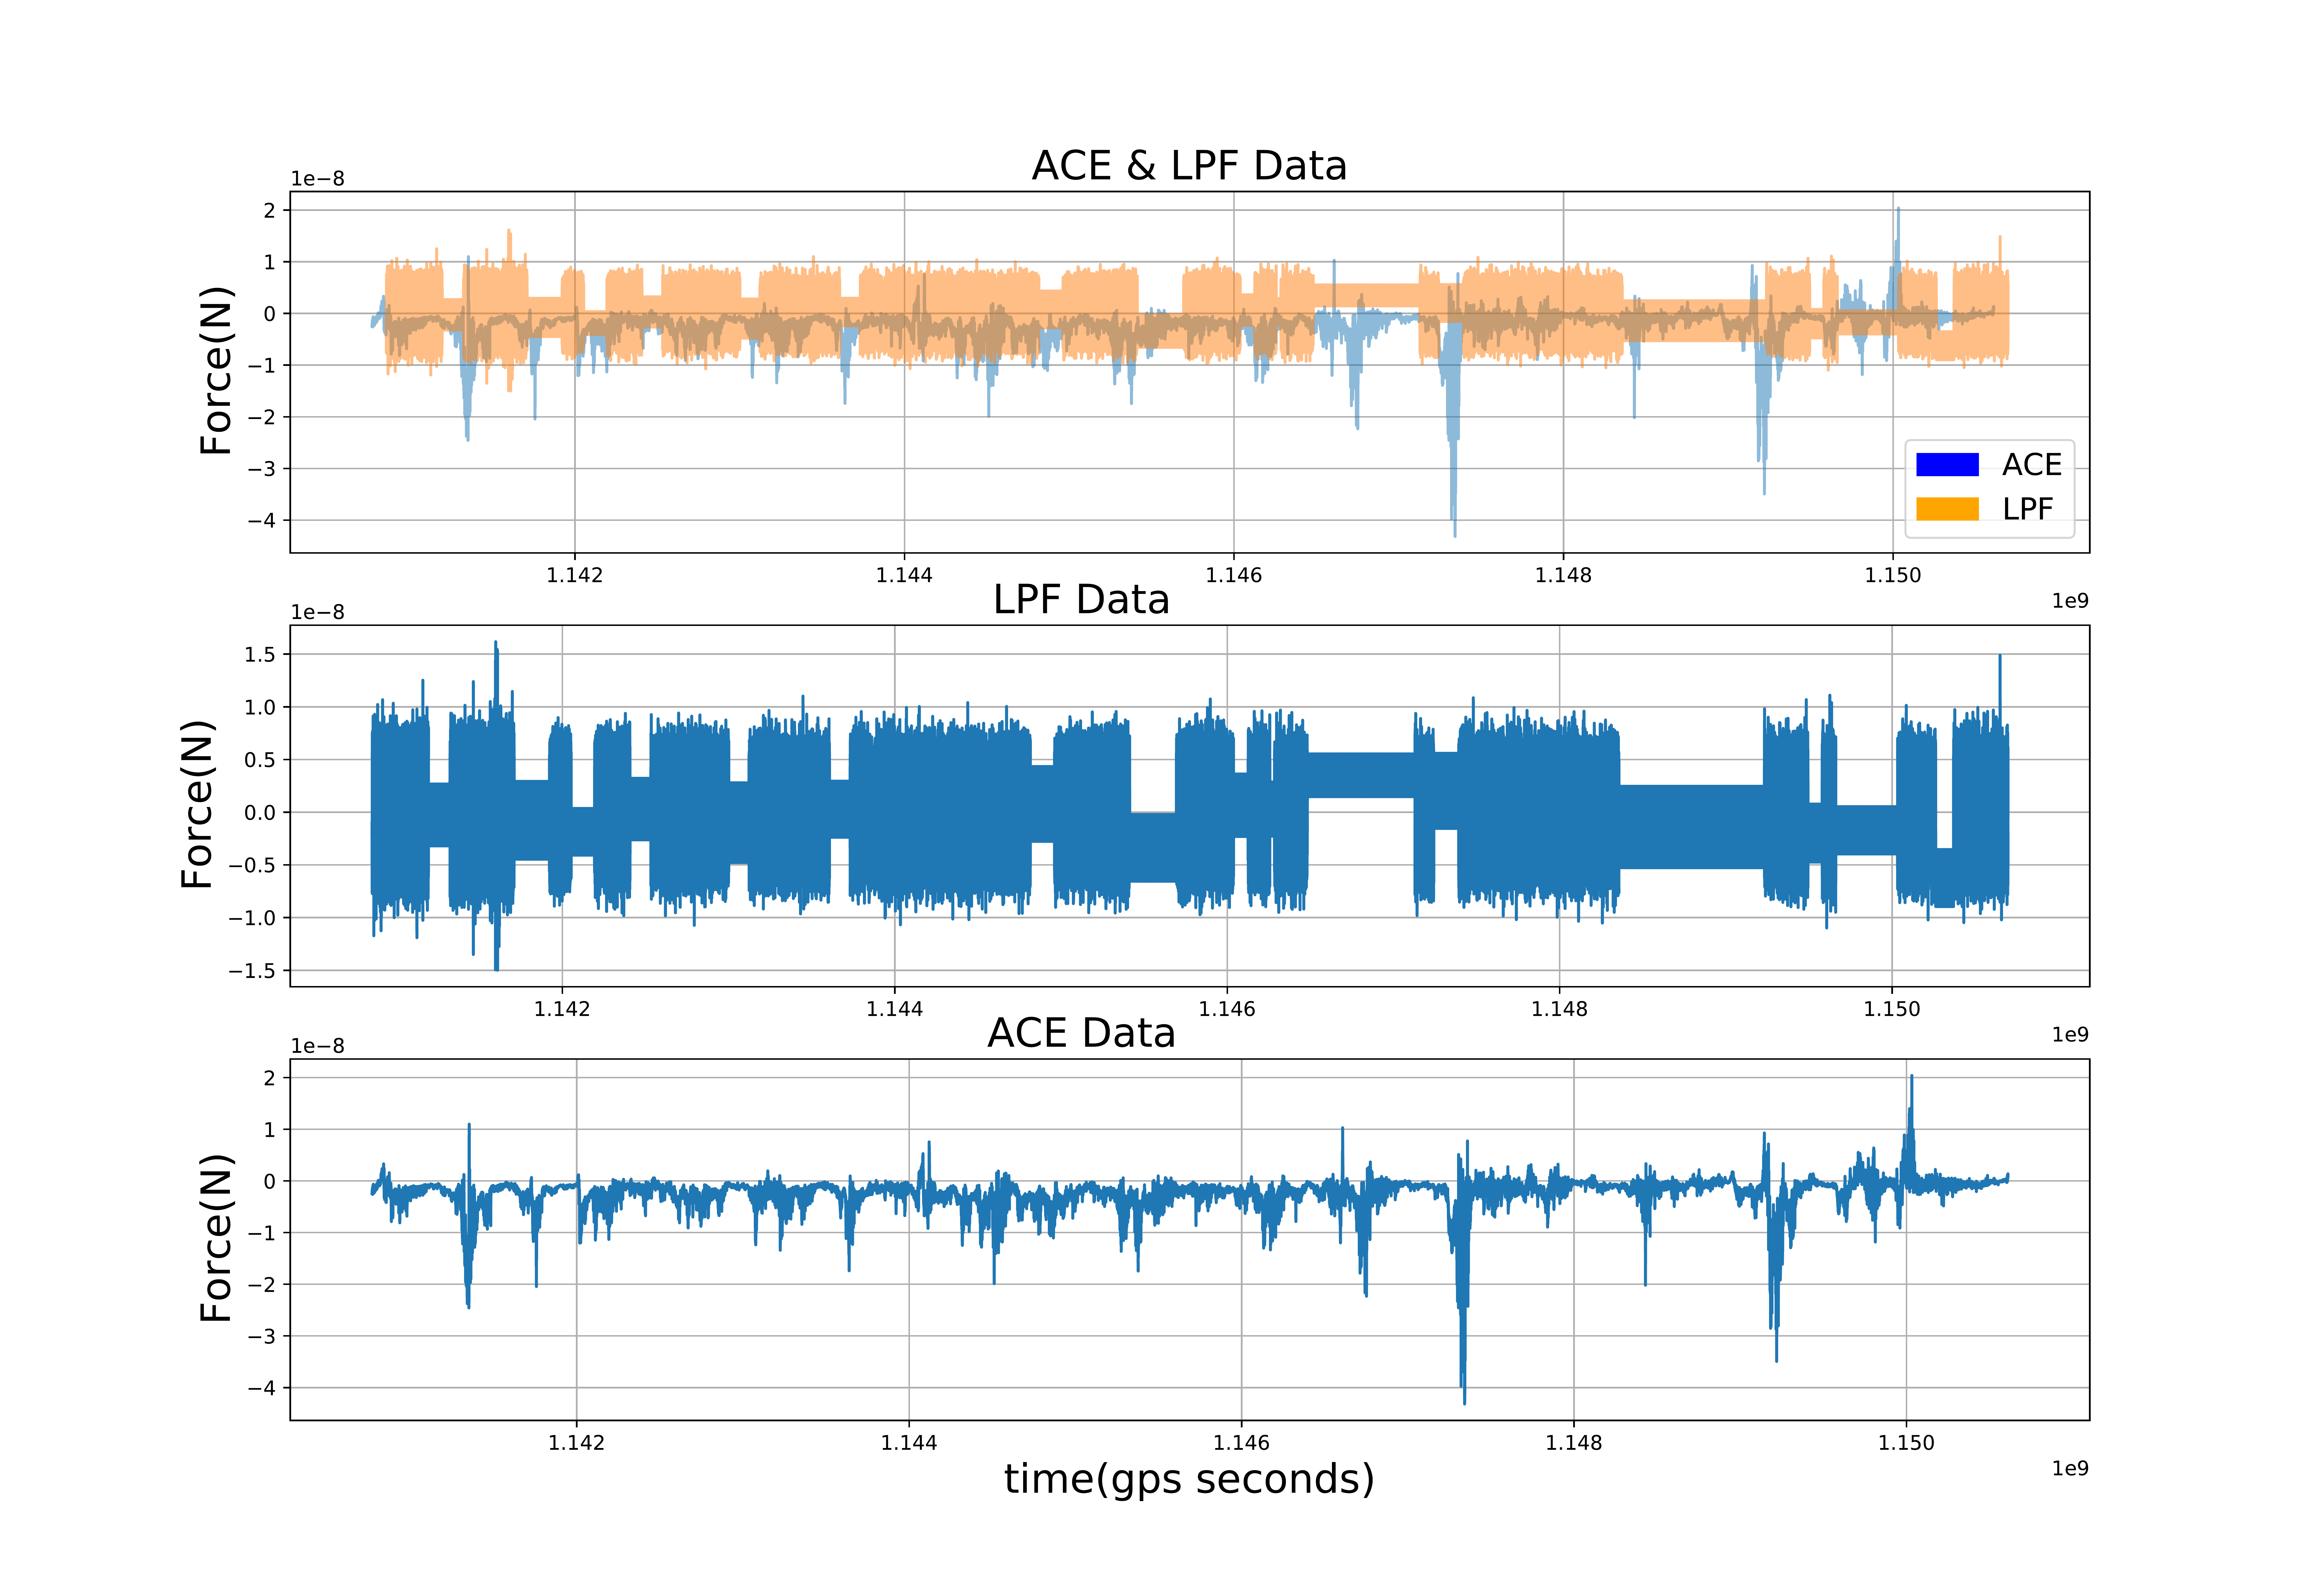
\includegraphics[width=0.5\textwidth]{TimeDomain_Comparison_ACEvLPF-1.png}}
\caption{Time series plot of ACE and LPF}
\label{fig}
\end{figure}
\begin{figure}[htbp]
\centerline{\includegraphics[width=0.5\textwidth]{ACE_and_LPF_loglo-1.png}}
\caption{FFT plot of ACE and LPF on a log-log scale}
\label{fig}
\end{figure}


\begin{figure}[htbp]
\centerline{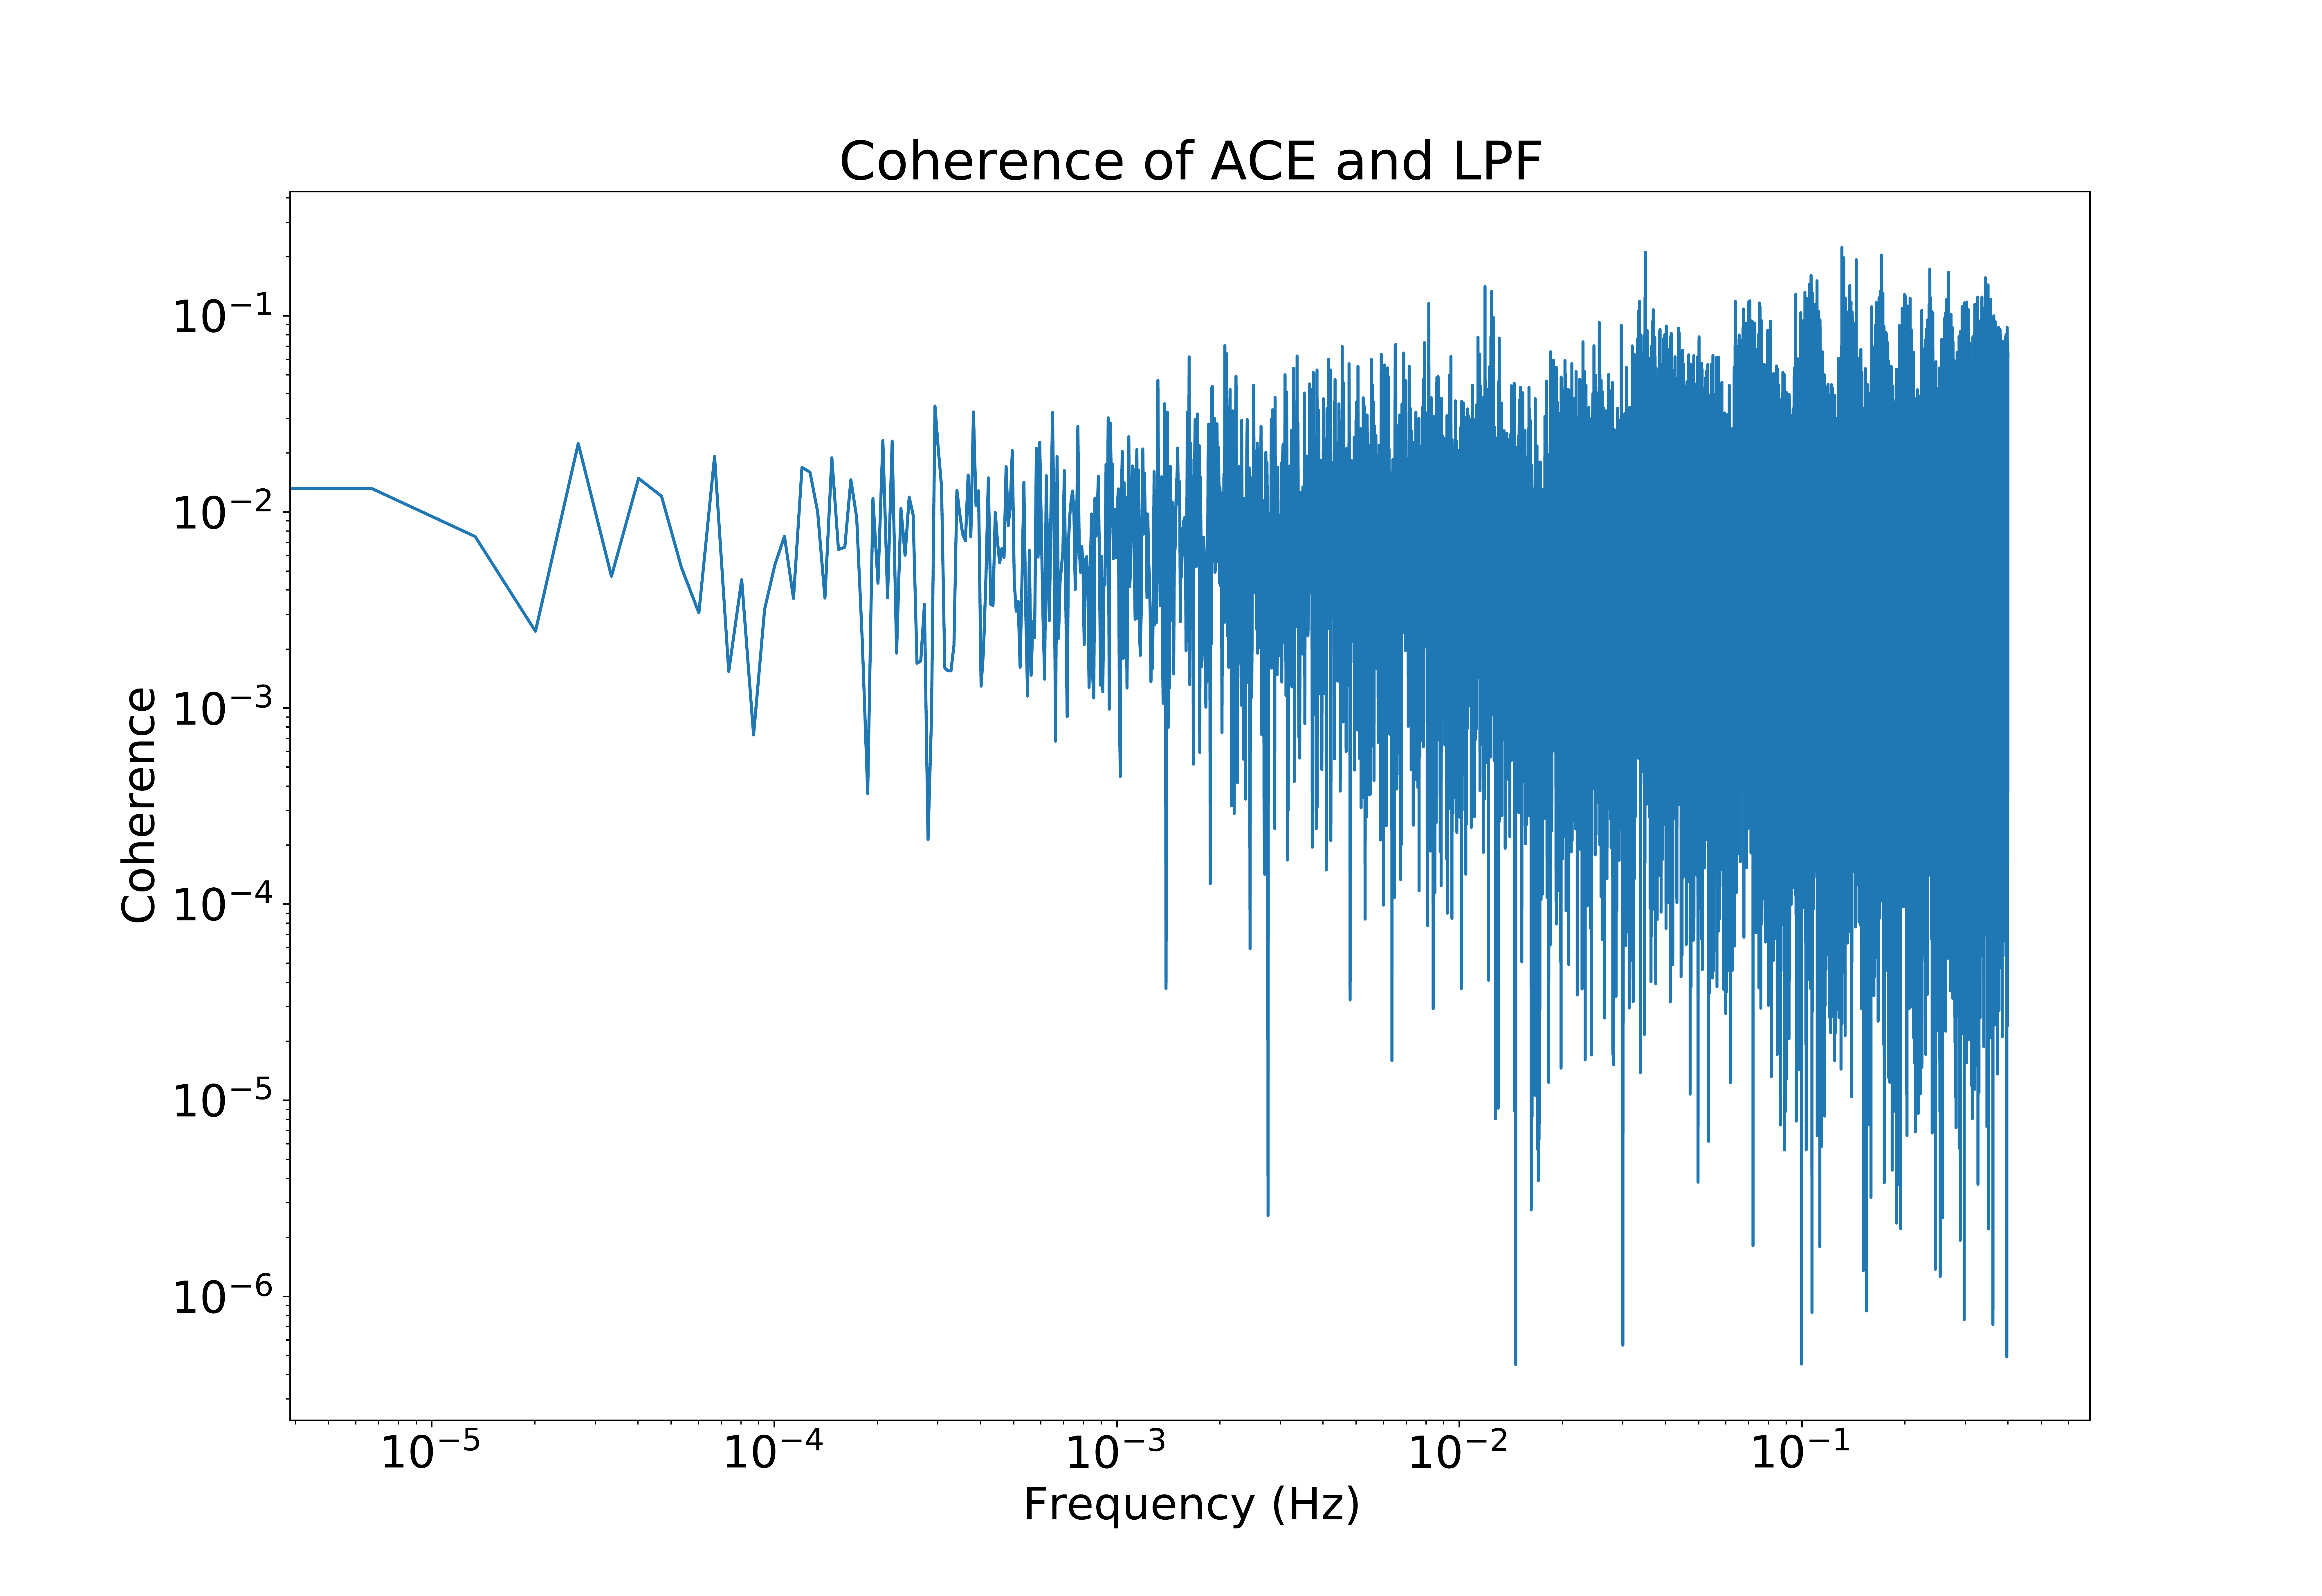
\includegraphics[width=0.5\textwidth]{ACE_and_LPF_co-1}}
\caption{Coherence plot of ACE and LPF}
\label{fig}
\end{figure}

\begin{figure}[htbp]
\centerline{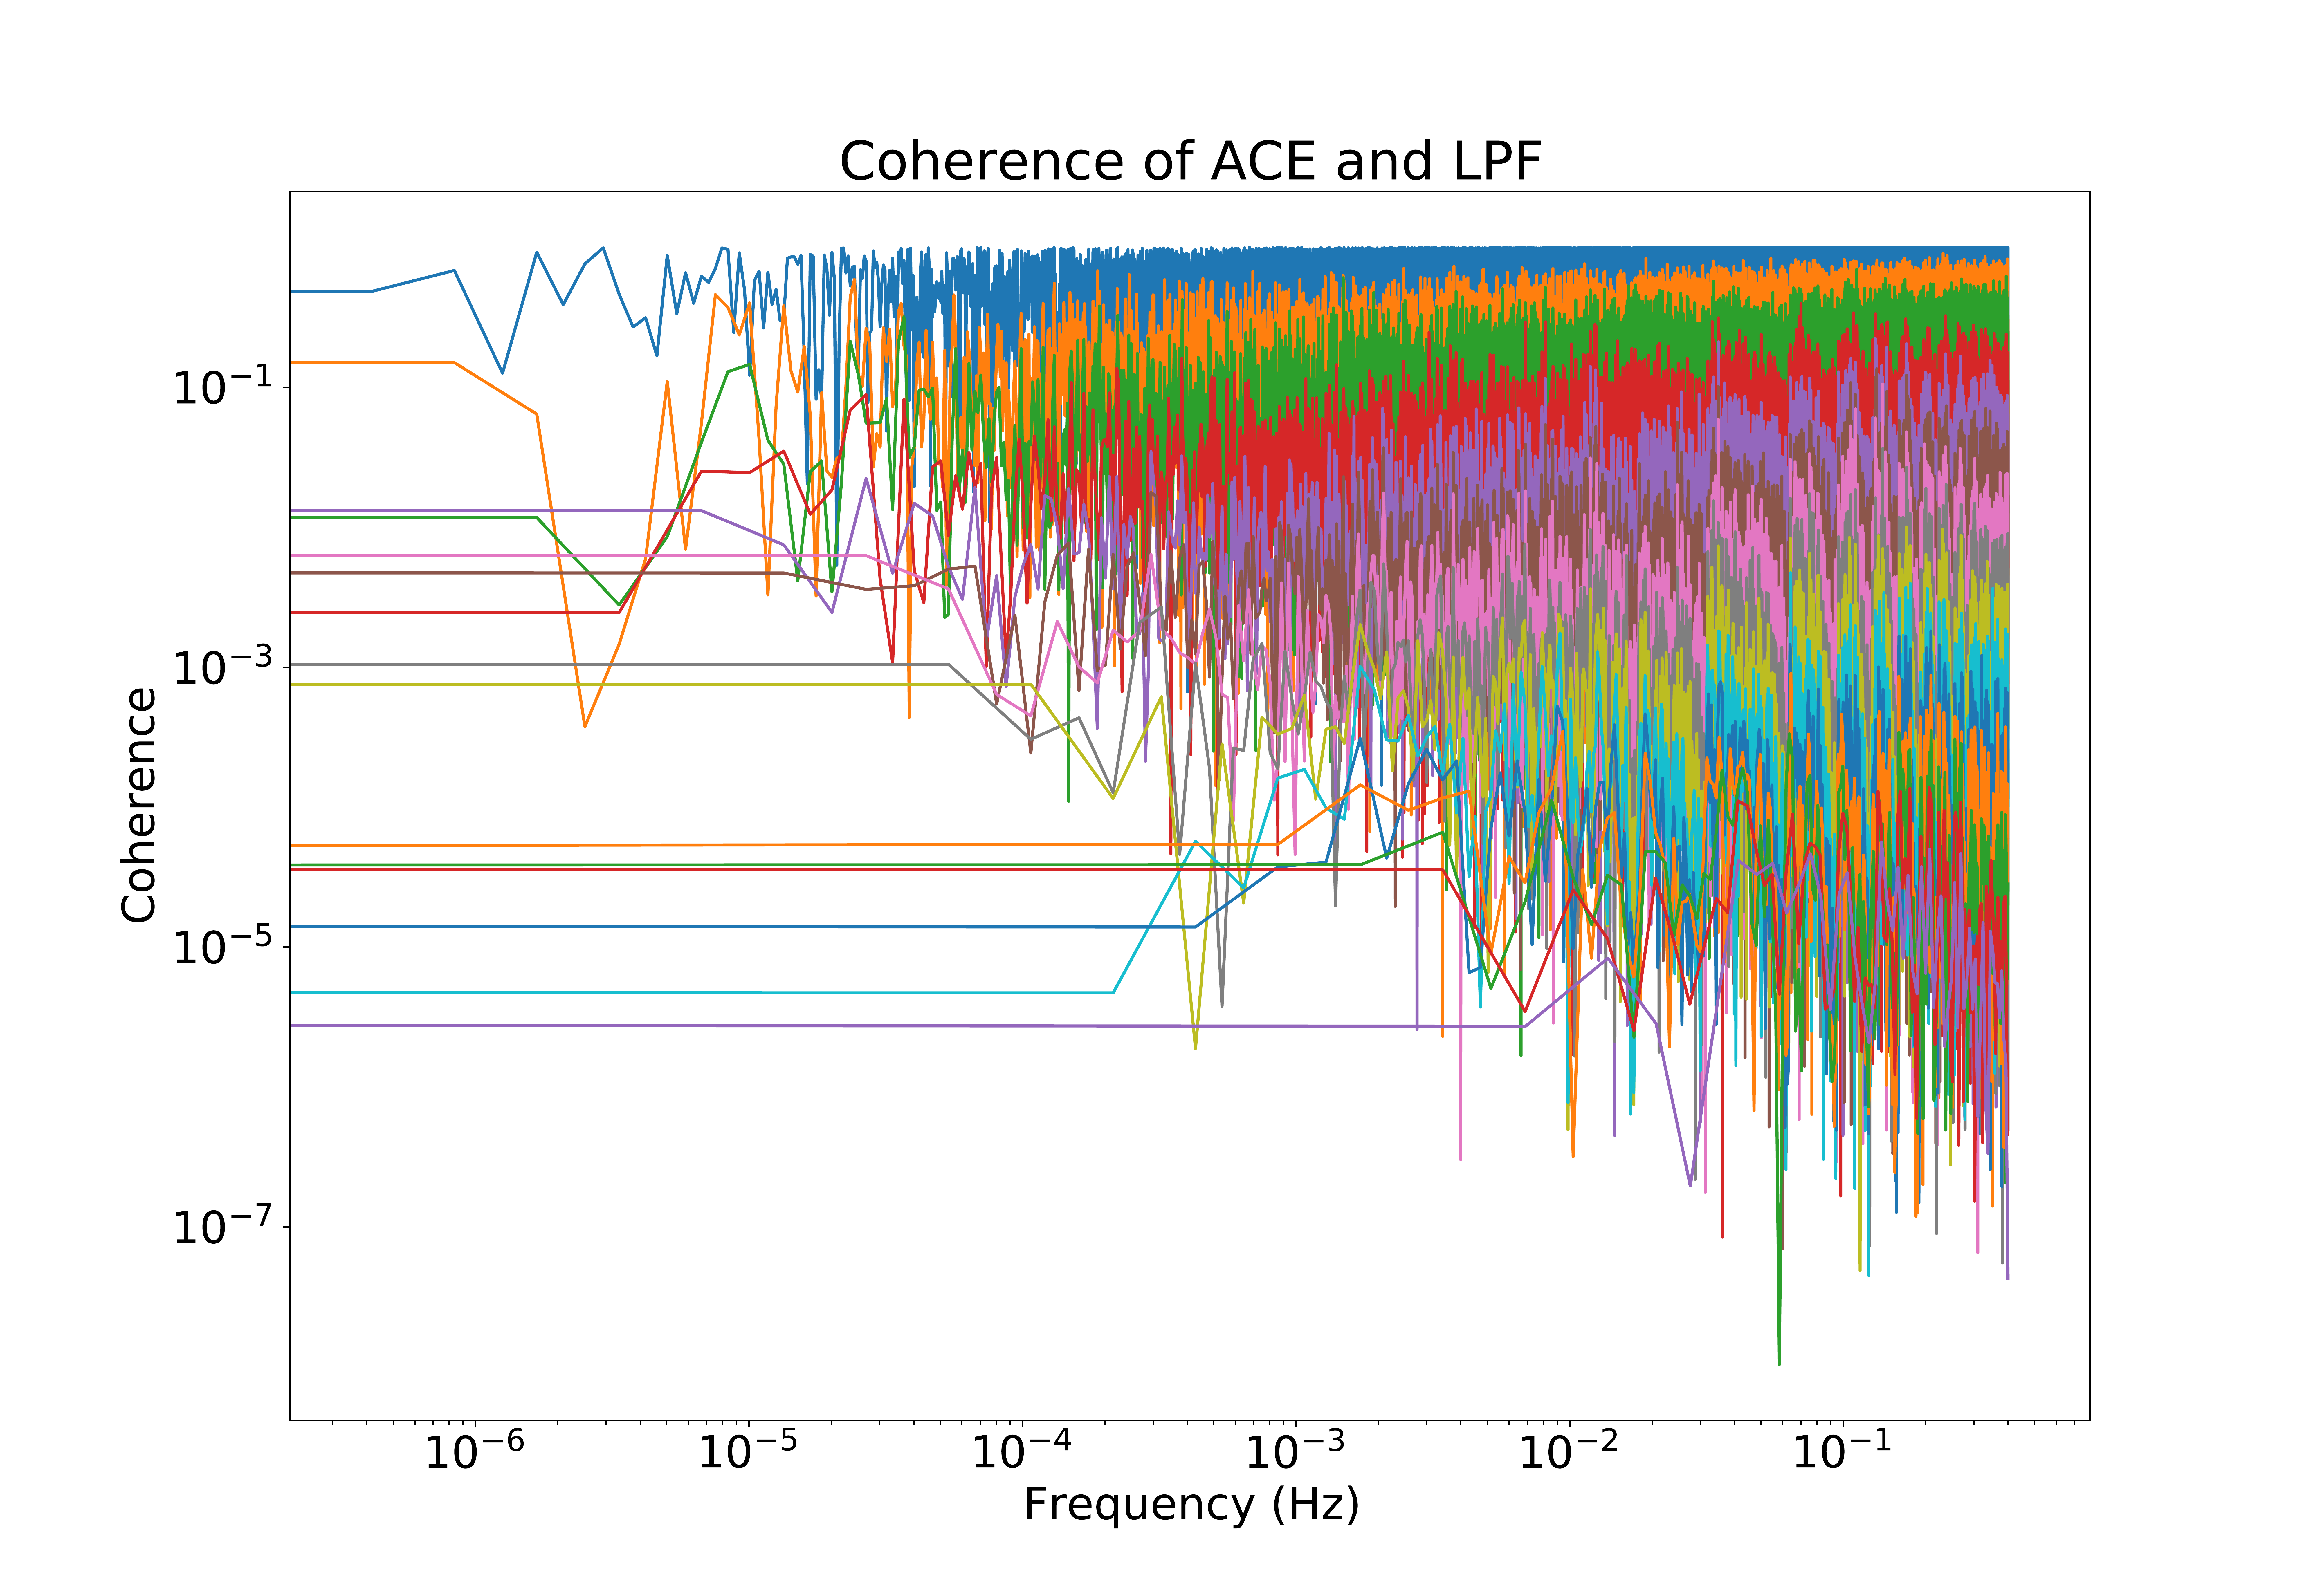
\includegraphics[width=0.5\textwidth]{ACE_and_LPF_co_2xx15-1}}
\caption{Coherence plot of ACE and LPF}
\label{fig}
\end{figure}


\begin{figure}[htbp]
\centerline{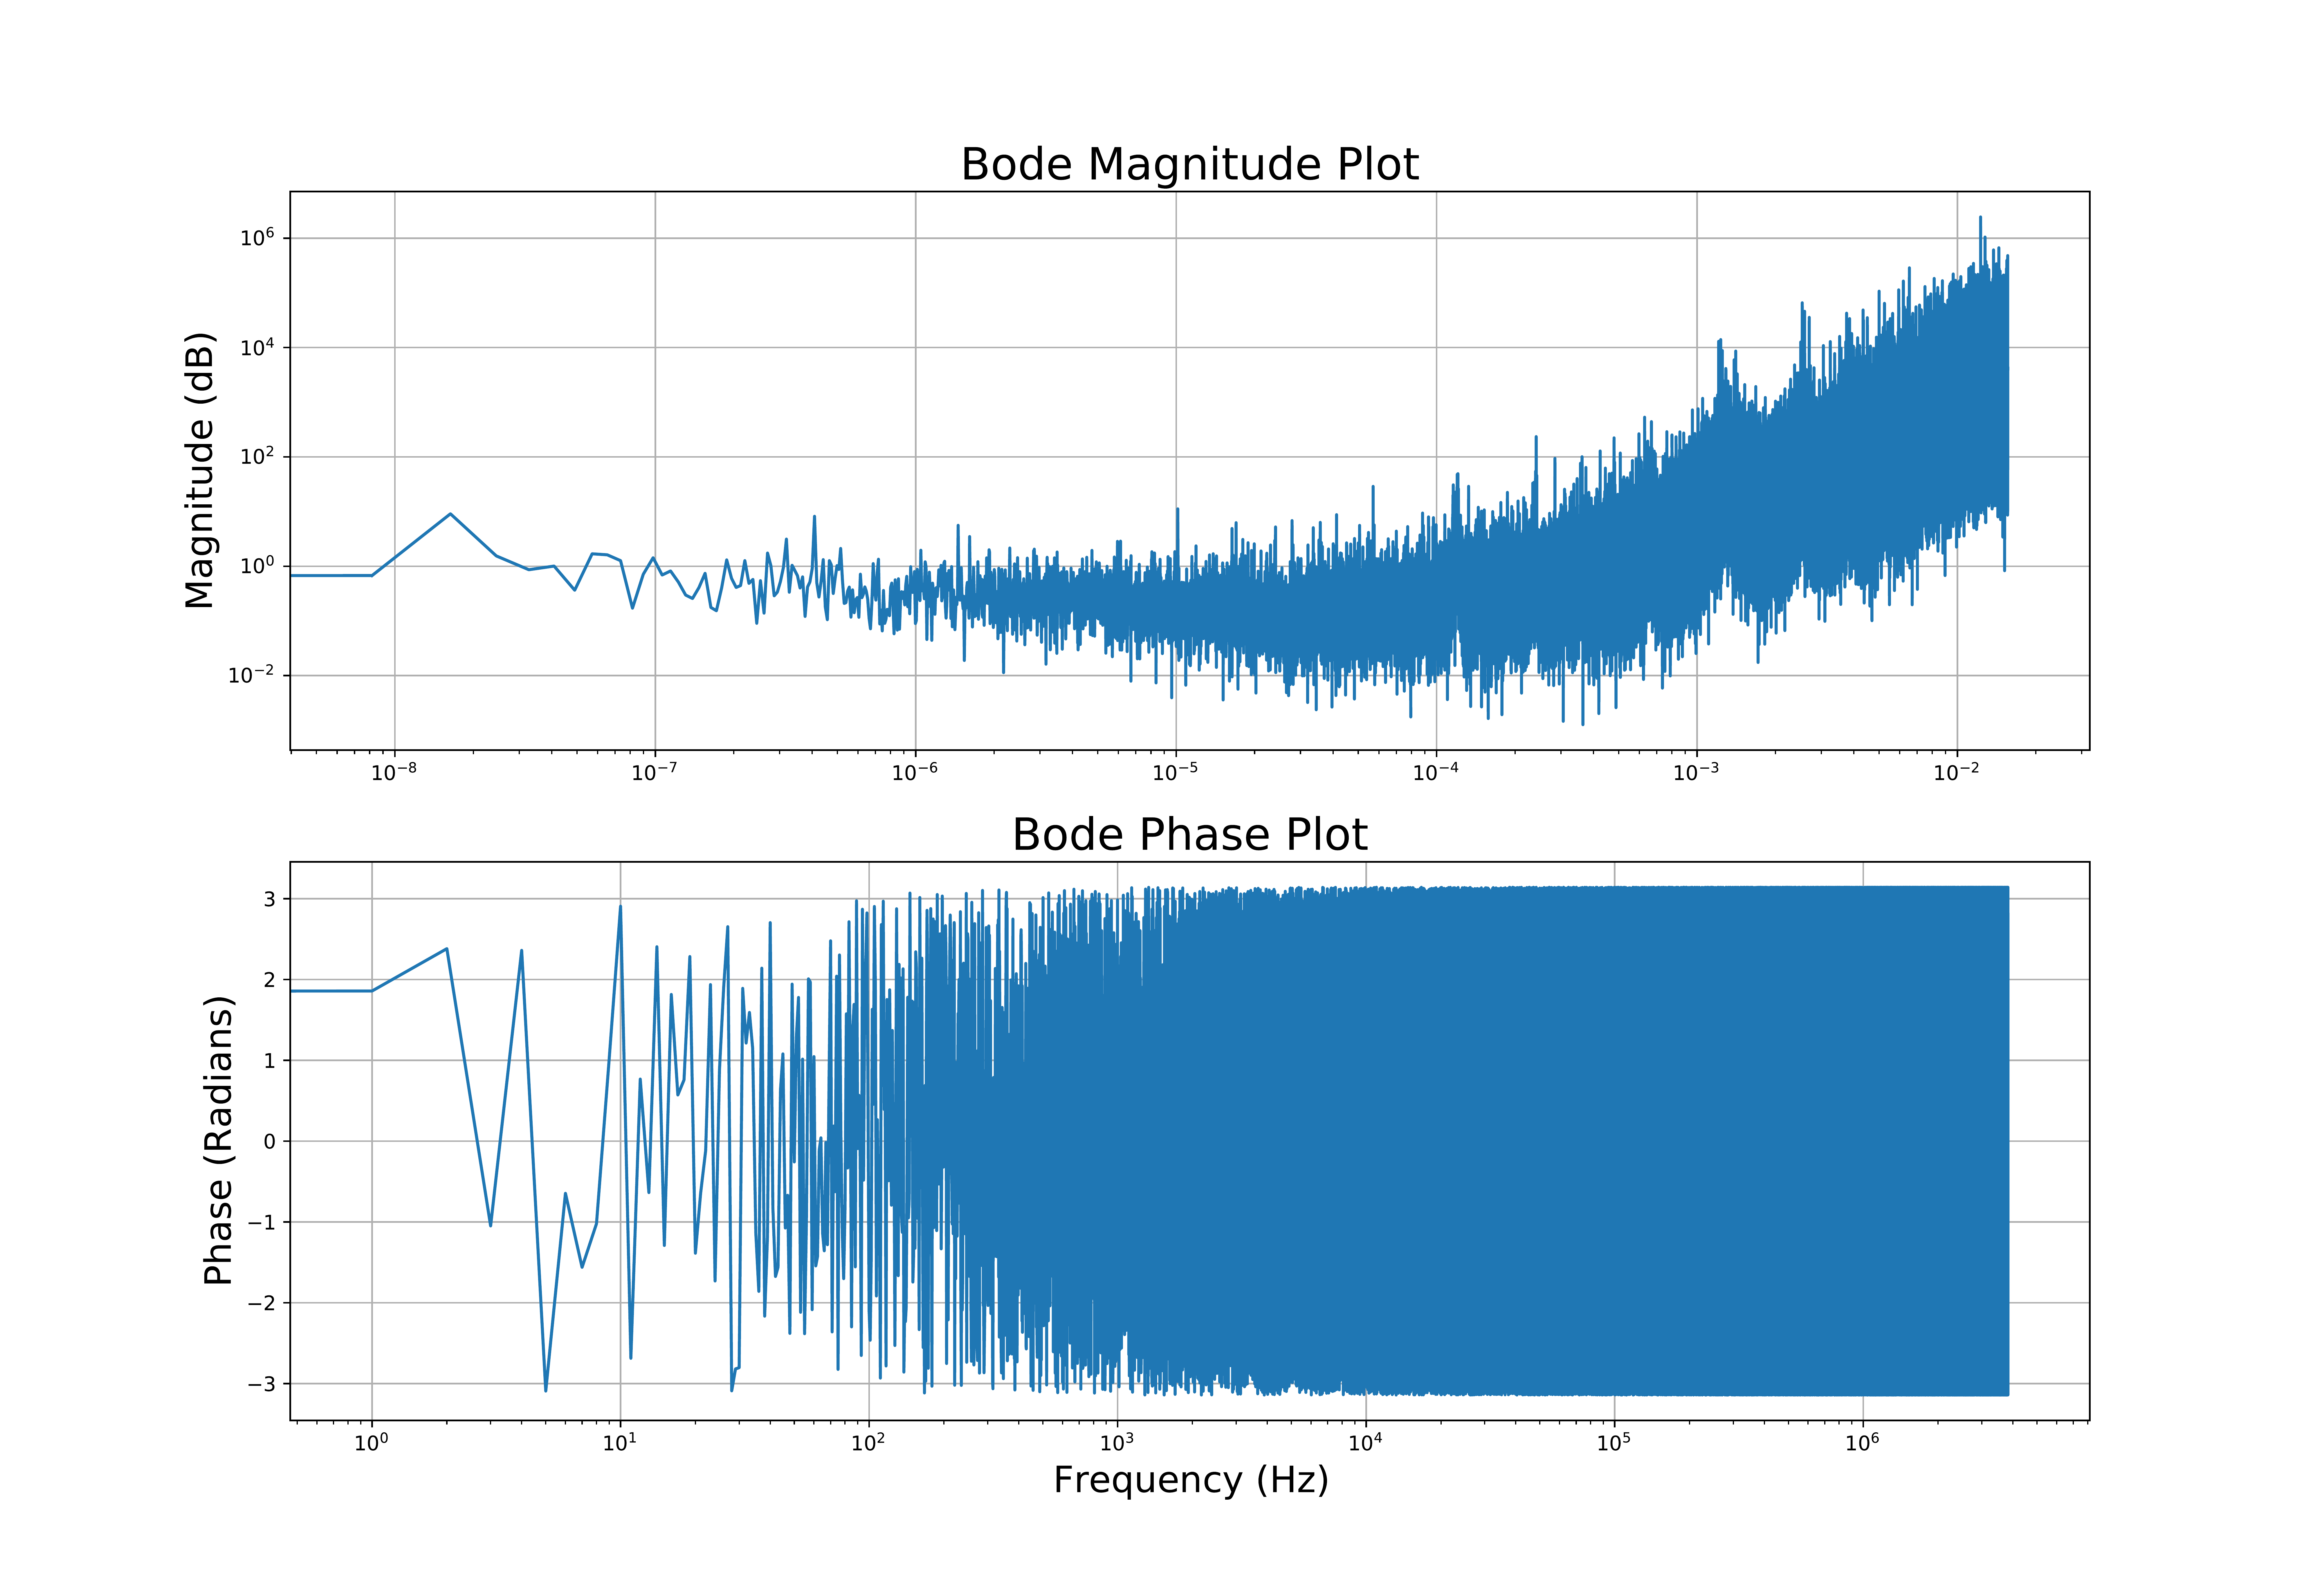
\includegraphics[width=0.5\textwidth]{Bode_plot-1.png}}
\caption{Bode magnitude plot}
\label{fig}
\end{figure}


\begin{figure}[htbp]
\centerline{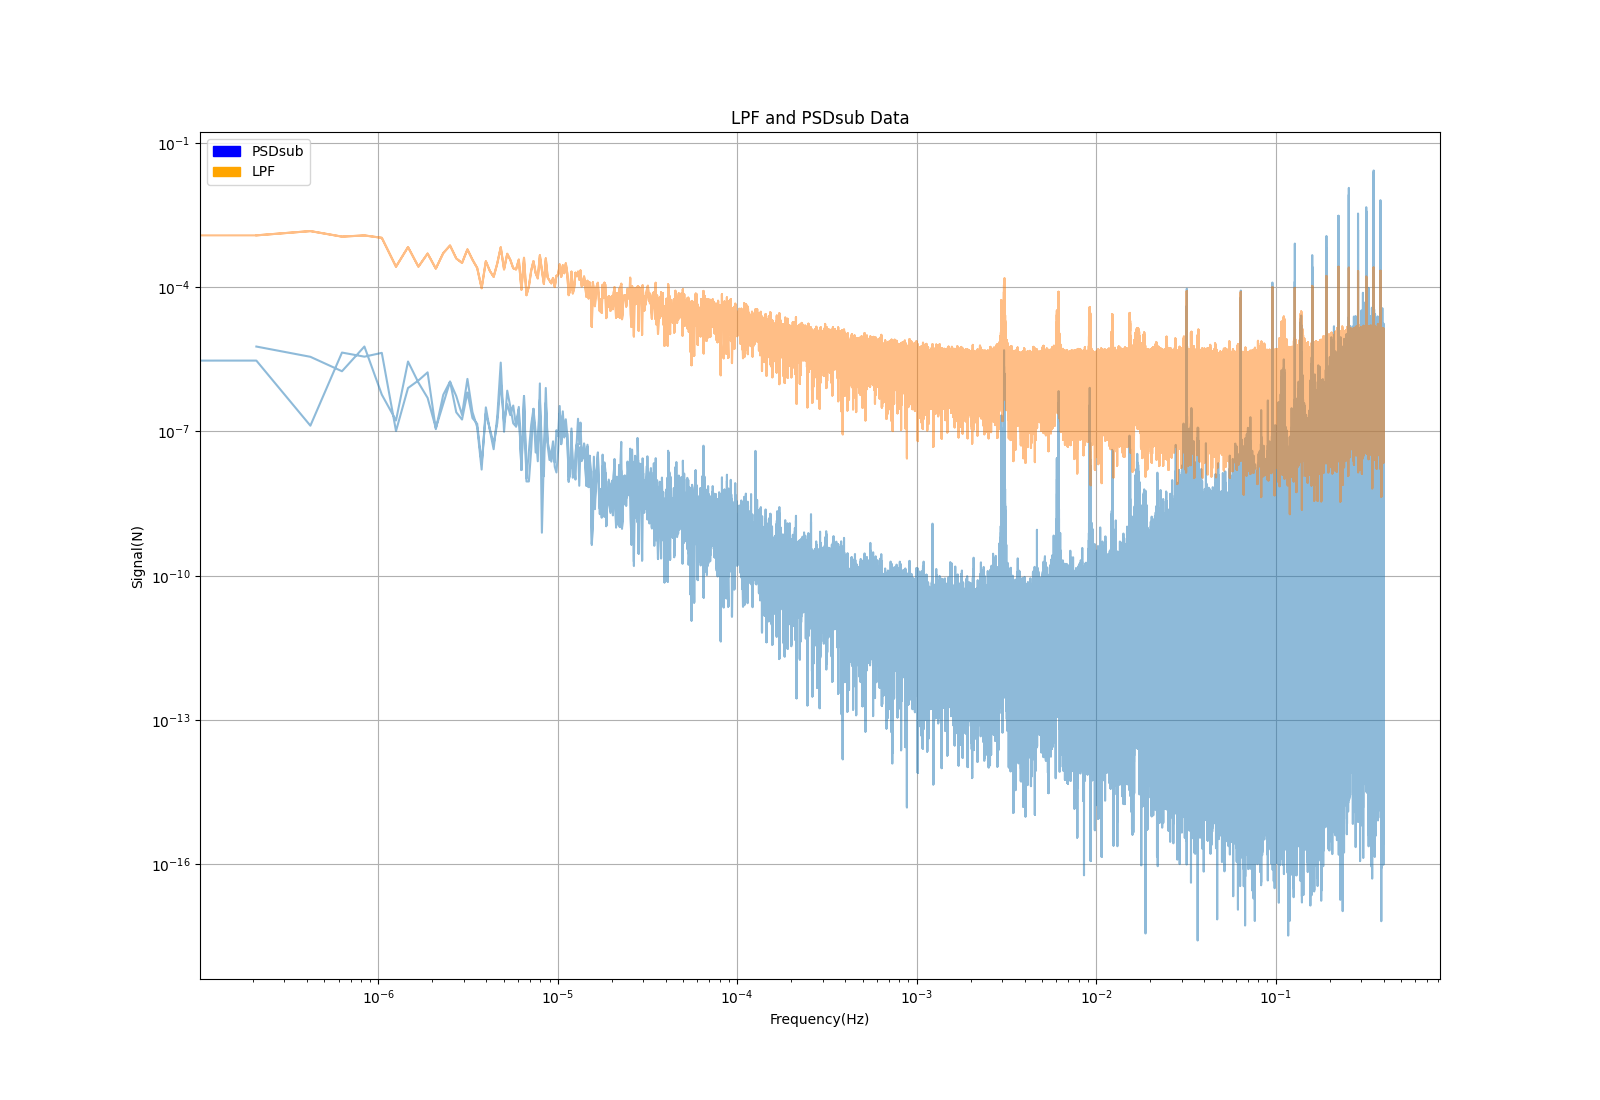
\includegraphics[width=0.5\textwidth]{LPF_Noise_Cancellation2.png}}
\caption{Noise cancellation plot of the original LPF data versus the original LPF data minus the spurious solar wind acceleration noise}
\label{fig}
\end{figure}


\section{Results}
The first plot(Fig 1.) made was a time series and from this plot we can see a direct comparison of LPF data time domain and ACE time domain, from this there isn't too much to conclude as there is too much noise in the Pathfinder data, therefore it will be easier to analyze after taking a FFT. 

In the FFT data log-log comparison plot(Fig. 4) it can be seen some minor similarities at certain points in the data, but the major spikes seem to not be seen in both graphs. To more directly compare them we created a Bode plot and a coherence plot which graphs the direct similarity between the 2 plots. 

A Bode Plot (Fig. 7) is the representation of the transfer function and from this it can be observed in the magnitude plot that the system is unstable and thus the 2 datasets don't correlate very well. 

From the coherence plot(Fig. 5) it was observed that the coherence between the 2 data sets was minimal and any correlation is probably due to random chance, and this was further tested in Fig. 6 where coherence plots average different lengths of correlation values. From the top to bottom the plots use increasing segment lengths by powers of 2 from 2 to \(2{^15}\). Thus this is great news for LISA as it will be able to collect much more data and we will be able to gain much more insight on the early universe. 

The final plot is a noise subplot, the orange represents the original LPF data and the blue represents the subtraction of the correlated noise between the ACE and LPF datasets from the original LPF data. Observing this plot, it didn't turn out as expected as the plot currently shows the subtractions as 3 magnitudes lower on the log-log scale. Therefore, that would suggest that the correlation between the 2 datasets would be about 90-99\%, currently the problem seems to be in the interpolation of the ACE dataset before the calculations between the 2. More work will need to be done in fixing this plot. 


\section{Conclusion}
The effects of spurious solar wind on acceleration noise of LPF data was thoroughly analyzed. The models and plots found little relation between the ACE solar wind data set and the Pathfinder to be minimal. This is encouraging for the future LISA and will allow the Pathfinder to see much more of the universe. As shown in Fig. 6, the coherence between the ACE and LPF data was sporadic for the given frequency range and the average correlation in Fig. 5 was minuscule. This shows that the correlation seen is mostly due to random chance and that so far there hasn't been any relationship found between ACE solar wind data and Pathfinder data. The first next step would be to experiment with the noise subtraction plot and deduce what's wrong.  For future tests, first since there is much gap fill across both data sets, it may be better to work on individual subsets and plot the relationships between those. Then, also try different force axis, for this the Z-axis was used for both the Pathfinder and the Solar wind velocity, however, the X-axis can also be used in comparing both data sets and it will be interesting to see whether or not solar wind has an affect on the ACE X-axis.


%\begin{acknowledgments}
%\end{acknowledgments}


% The \nocite command causes all entries in a bibliography to be printed out
% whether or not they are actually referenced in the text. This is appropriate
% for the sample file to show the different styles of references, but authors
% most likely will not want to use it.
\nocite{*}

\bibliography{apssamp}% Produces the bibliography via BibTeX.

\end{document}
%
% ****** End of file apssamp.tex ******
    